\begin{figure}
	\begin{minipage}
		{.5 
		\textwidth} \hspace{-15 mm} 
		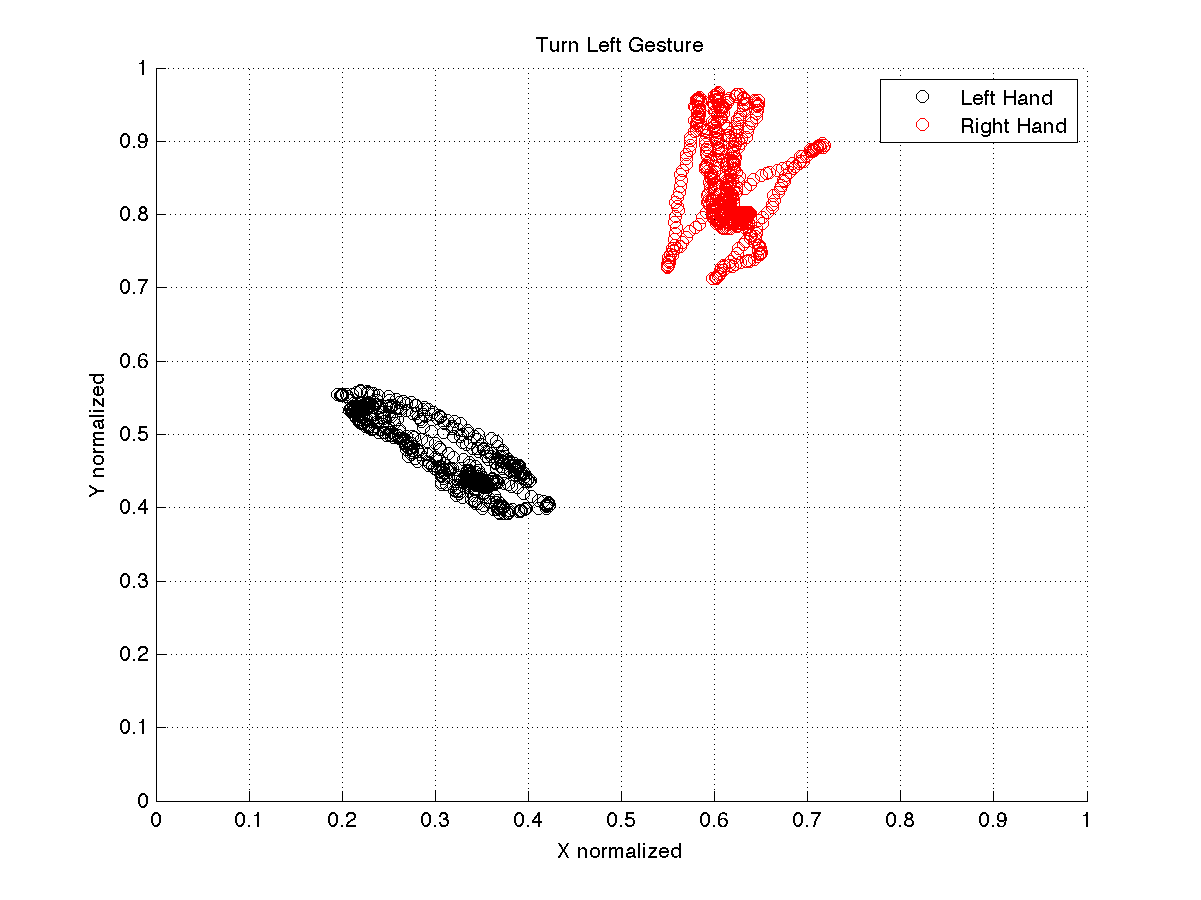
\includegraphics[height=70mm]{figures/result/train-turn-left.png} \caption*{Turn Left Gesture} 
	\end{minipage}
	\begin{minipage}
		{.5 
		\textwidth} 
		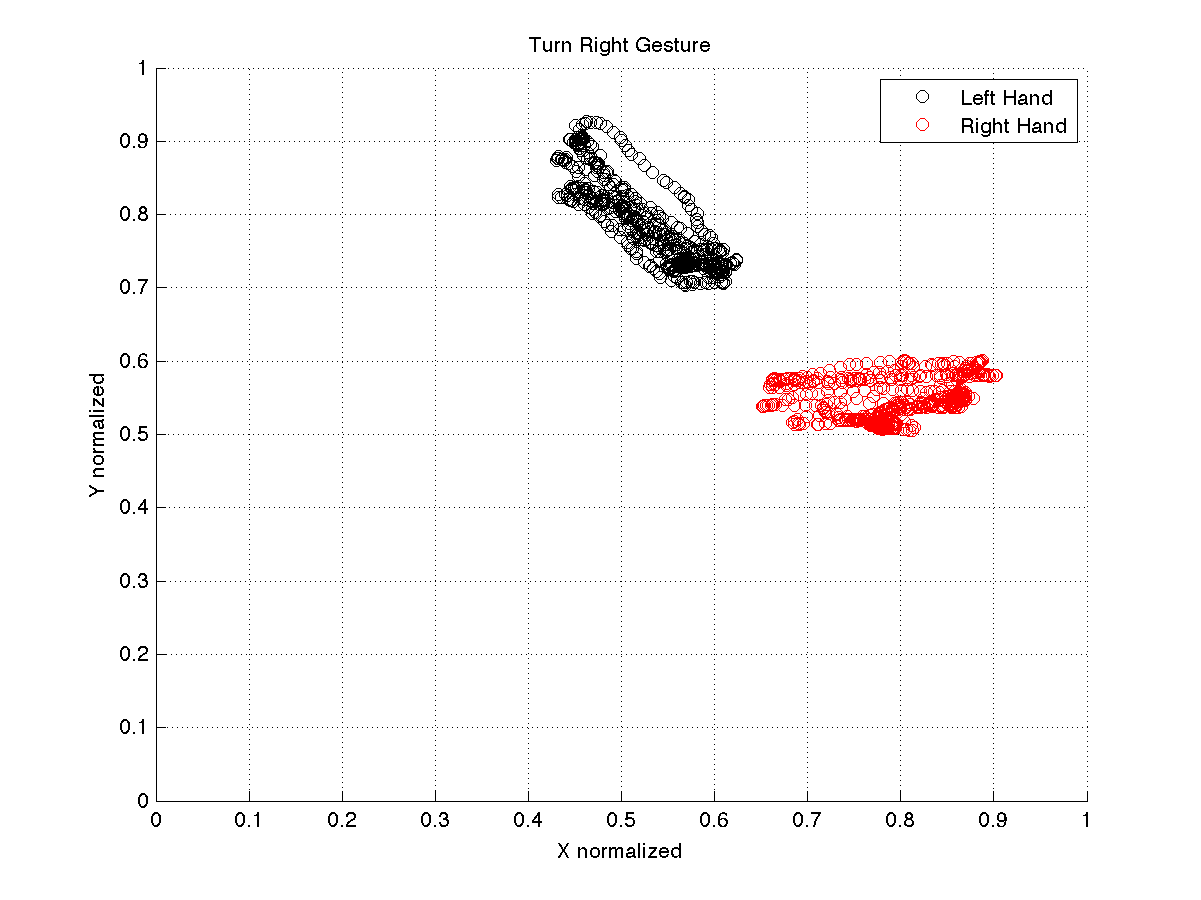
\includegraphics[height=70mm]{figures/result/train-turn-right.png} \caption*{Turn Right Gesture} 
	\end{minipage}
	\begin{minipage}
		{.5 
		\textwidth} \hspace{-15 mm} 
		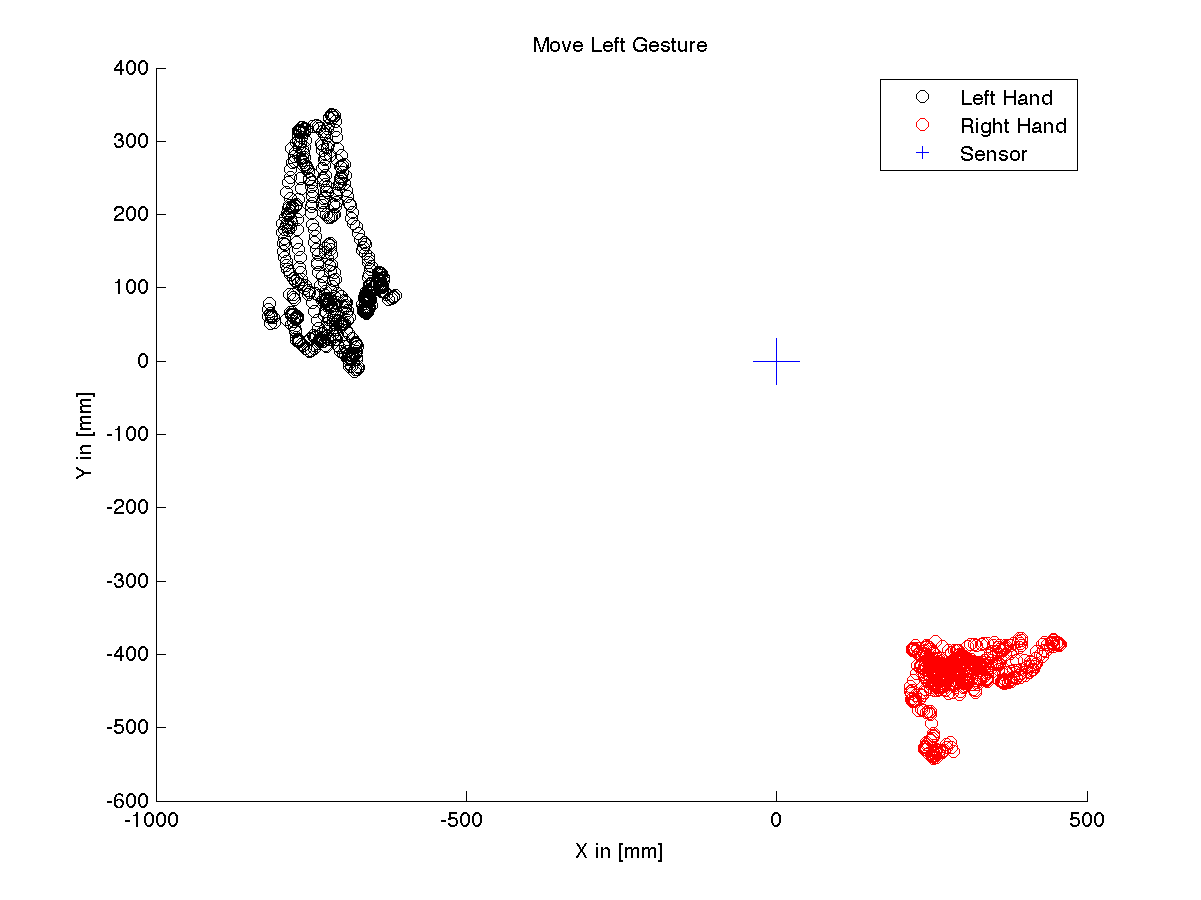
\includegraphics[height=70mm]{figures/result/train-move-left.png} \caption*{Move Left Gesture} 
	\end{minipage}
	\begin{minipage}
		{.5 
		\textwidth} 
		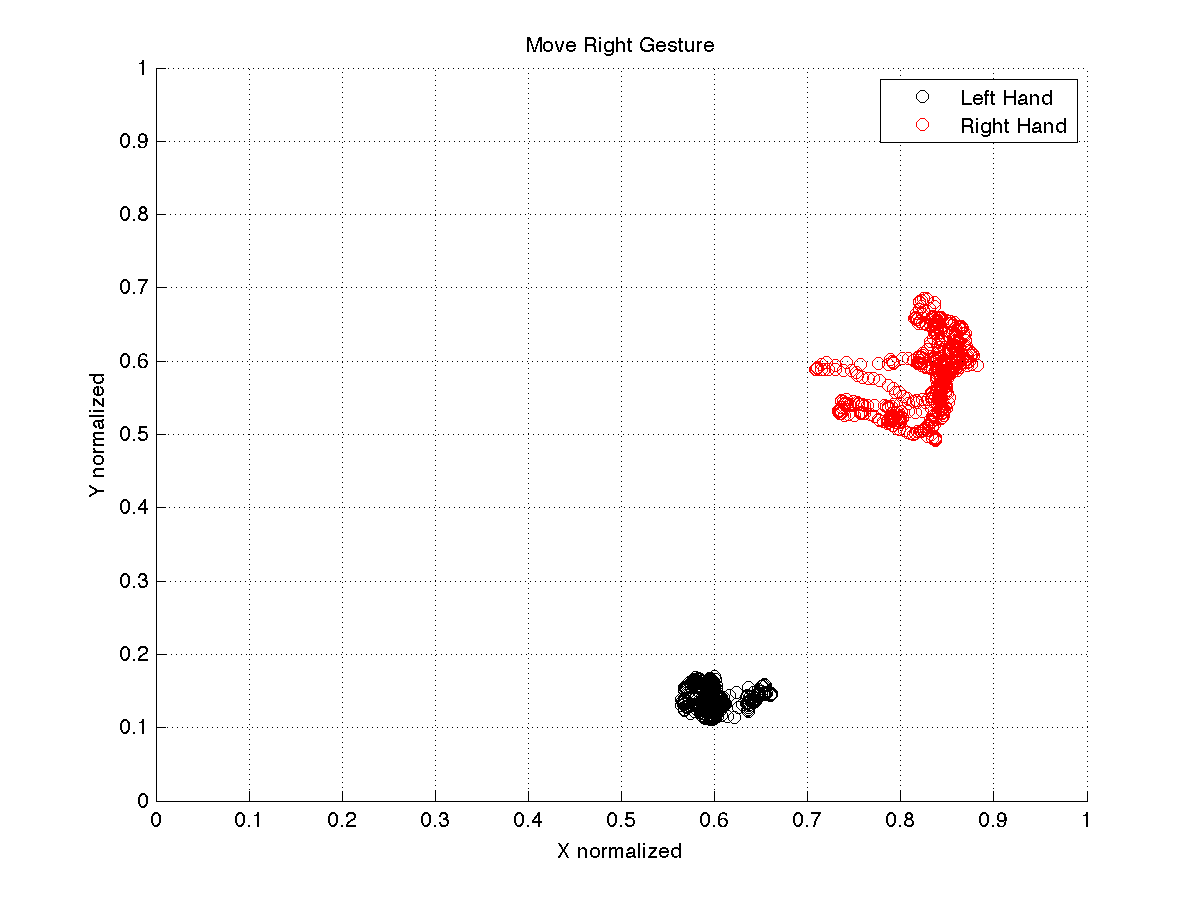
\includegraphics[height=70mm]{figures/result/train-move-right.png} \caption*{Move Right Gesture} 
	\end{minipage}
	\begin{minipage}
		{.5 
		\textwidth} \hspace{-15 mm} 
		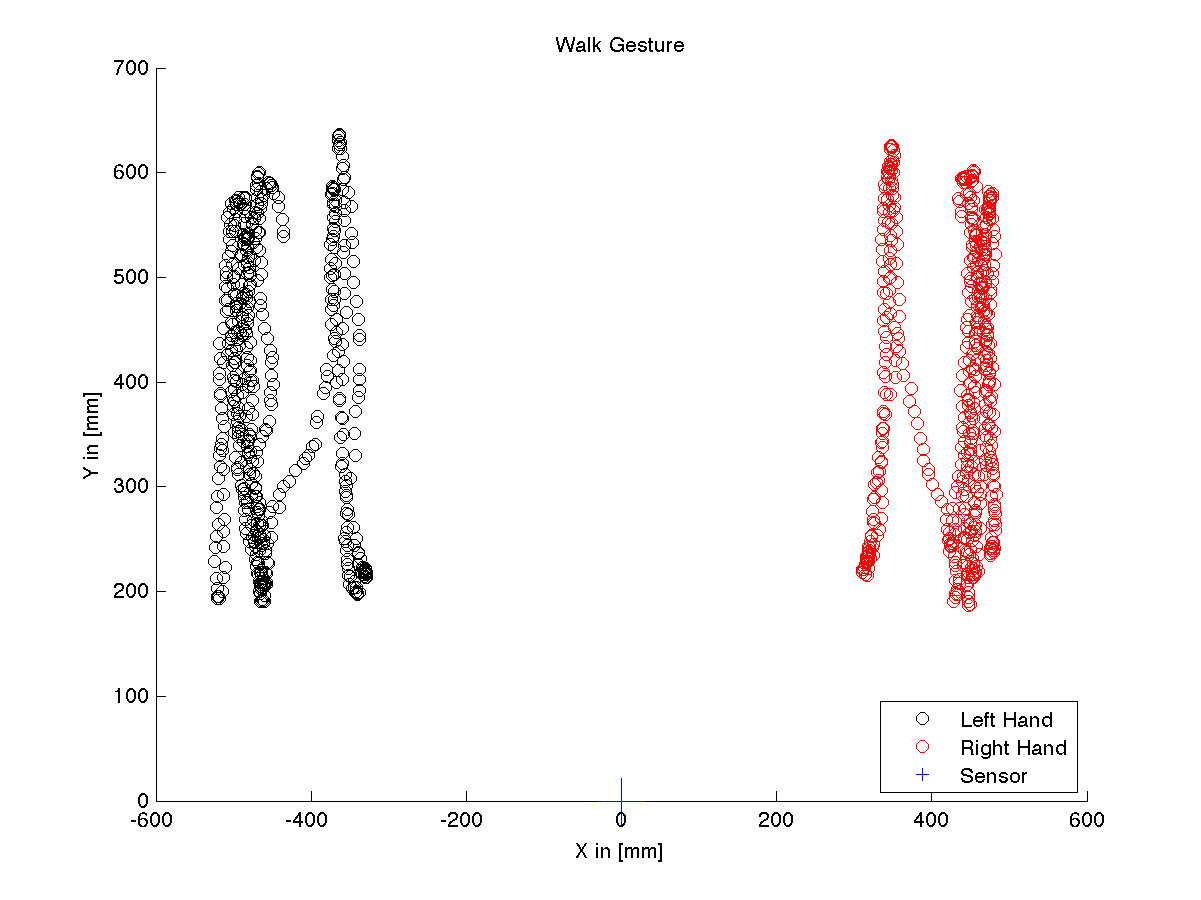
\includegraphics[height=70mm]{figures/result/train-walk.png} \caption*{Walk Gesture} 
	\end{minipage}
	\caption{Normalized training dataset of all 5 gestures are plotted in x and y axis to show that the position of hands are moved during the recording time to get more variations of the same gesture.} \label{pl:ges:pos} 
\end{figure}
